%!TEX root = ../../main.tex

\chapter{Theoretische Grundlagen}

\section{Unwucht}
Eine Unwucht ist eine Rotation, welche bei einem rotierenden Körper nicht in der Hauptträgheitsachse stattfindet, sondern leicht versetzt.
Diese Versetzung führt zu drehzahlabhängigen Vibrationen, welche zu einem erhöhten Verschleiss, bis hin zu der Zerstörung des gesamten Systems führen können.
Eine Unwucht bei einem Rotationskörper ensteht, wenn sich der Schwerpunkt des Körpers nicht auf der Rotationsachse befindet und damit die Fliehkräfte nicht mehr gegenseitig aufgehoben werden können.

Es wird zwischen zwei Arten von Unwuchten unterschieden:
\begin{itemize}
	\item Statische Unwucht
	\item Dynamische Unwucht
\end{itemize}

Die statische Unwucht entsteht, wenn an einem vollkommen ausgewuchteten Rotationskörper auf der Radialebene eine Schwerpunktverlagerung stattfindet.
Dadurch entstehen kreisförmige Schwingungen rechtwinklig zur Rotationsachse.
\begin{figure}[H]
	\centering
	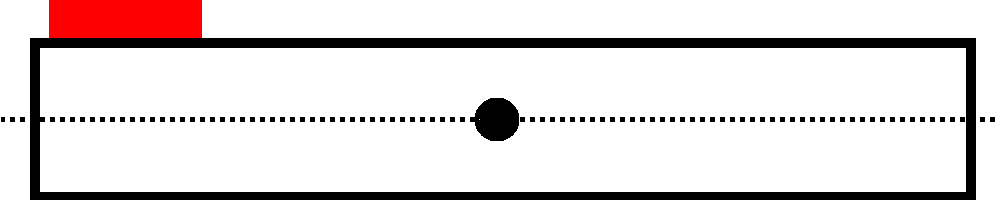
\includegraphics[width=5cm]{images/chapter/02/static_imbalance.png}
	\caption{Bildliche Darstellung einer statischen Unwucht}
\end{figure}
Die dynamische Unwucht hingegen tritt auf, wenn sich zwei gleich große, aber zueinander entgegengesetzt liegende Unwuchten in unterschiedlichen Radialebenen befinden.
Hierdurch fängt die Rotationsachse an zu taumeln, während der Schwerpunkt des Rotationskörpers in Ruhelage verbleibt.
Diese Art der Unwucht macht sich jedoch erst bei sehr schnellen Drehzahlen bemerkbar.
\begin{figure}[H]
	\centering
	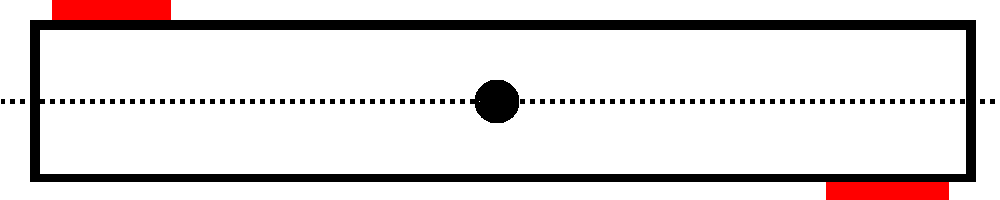
\includegraphics[width=5cm]{images/chapter/02/dynamic_imbalance.png}
	\caption{Bildliche Darstellung einer dynamischen Unwucht}
\end{figure}

\section{Mikrocontrollerplattform Arduino}
